\section{Results}
\label{sec:evaluation:results}

In this section, we discuss the results of our findings from the evaluation strategies proposed in \cref{sec:evaluation:strategies} using the metrics described in \cref{sec:background:metrics,sec:evaluation:metrics}. We also discuss limitations of the pipeline and possible mitigations.

\subsection{Summarised Performance over all Evaluations}
\label{sec:evaluation:results}

Presented in \cref{fig:evaluation:results:performance_all} are the bib, text and character performance collated of all 16 evaluations. These values were calculated at a post-evaluation stage by comparing the output results with the ground truth. For further results, refer to \cref{tab:results:summary:bib,tab:results:summary:text,tab:results:summary:ocr}. For bib region accuracies detected by the pipeline, a mean \fscore{} 0.14 is observed for ideal cases and 0.07 for realistic cases. A comparison between cropping and not cropping in both evaluation sets is presented in \cref{tab:evaluation:fscore_comparison}.

Generally, not cropping improves the \fscore{} value in both evaluation sets, though our performance in the ideal cases are improved due to an increased false negative rate observed in the realistic cases (i.e., generally not all bibs are detected when there are more than one runner). This is most likely caused by the randomised dataset used to evaluate our pipeline as well as the quality of tagging made of ground truth accuracies on our pipeline: should a dataset of photos that have only been \textit{sold} (and thus implicitly imply a greater prominence of the runner within each photo) with more fine-tuned tagging using Argus, we suggest that these detection rates would improve. We leave such evaluations up for future work.

\begin{table}[h]
\centering
\caption[Comparison of our \fscore{} results]{Comparison of various \fscore{} values for cropping versus evaluation sets.}
\label{tab:evaluation:fscore_comparison}
\begin{tabular}{lll}
\hline
\multicolumn{1}{c}{\multirow{2}{*}{\textbf{Evaluation Set}}} & \multicolumn{2}{c}{\textbf{Cropping}} \\ \cline{2-3} 
\multicolumn{1}{c}{}                                         & Yes                & No               \\ \hline
Ideal                                                        & 0.11               & 0.17             \\ 
Realistic                                                    & 0.03               & 0.10             \\ \hline
\end{tabular}
\end{table}

We note the model performance is positively associated with the amount of training data supplied, and the significant improvement that \textit{not} cropping on humans makes. Therefore, we conclude that this reduction is caused by the association that \frcnn{} has made of a bib sheet to a human torso: it is likely that the network recognises these bib sheets best when the raw input is provided as this is the augmented dataset that we trained our network on (i.e., we did not train our network on cropped humans).

\begin{landscape}

\begin{figure}
  \centering
  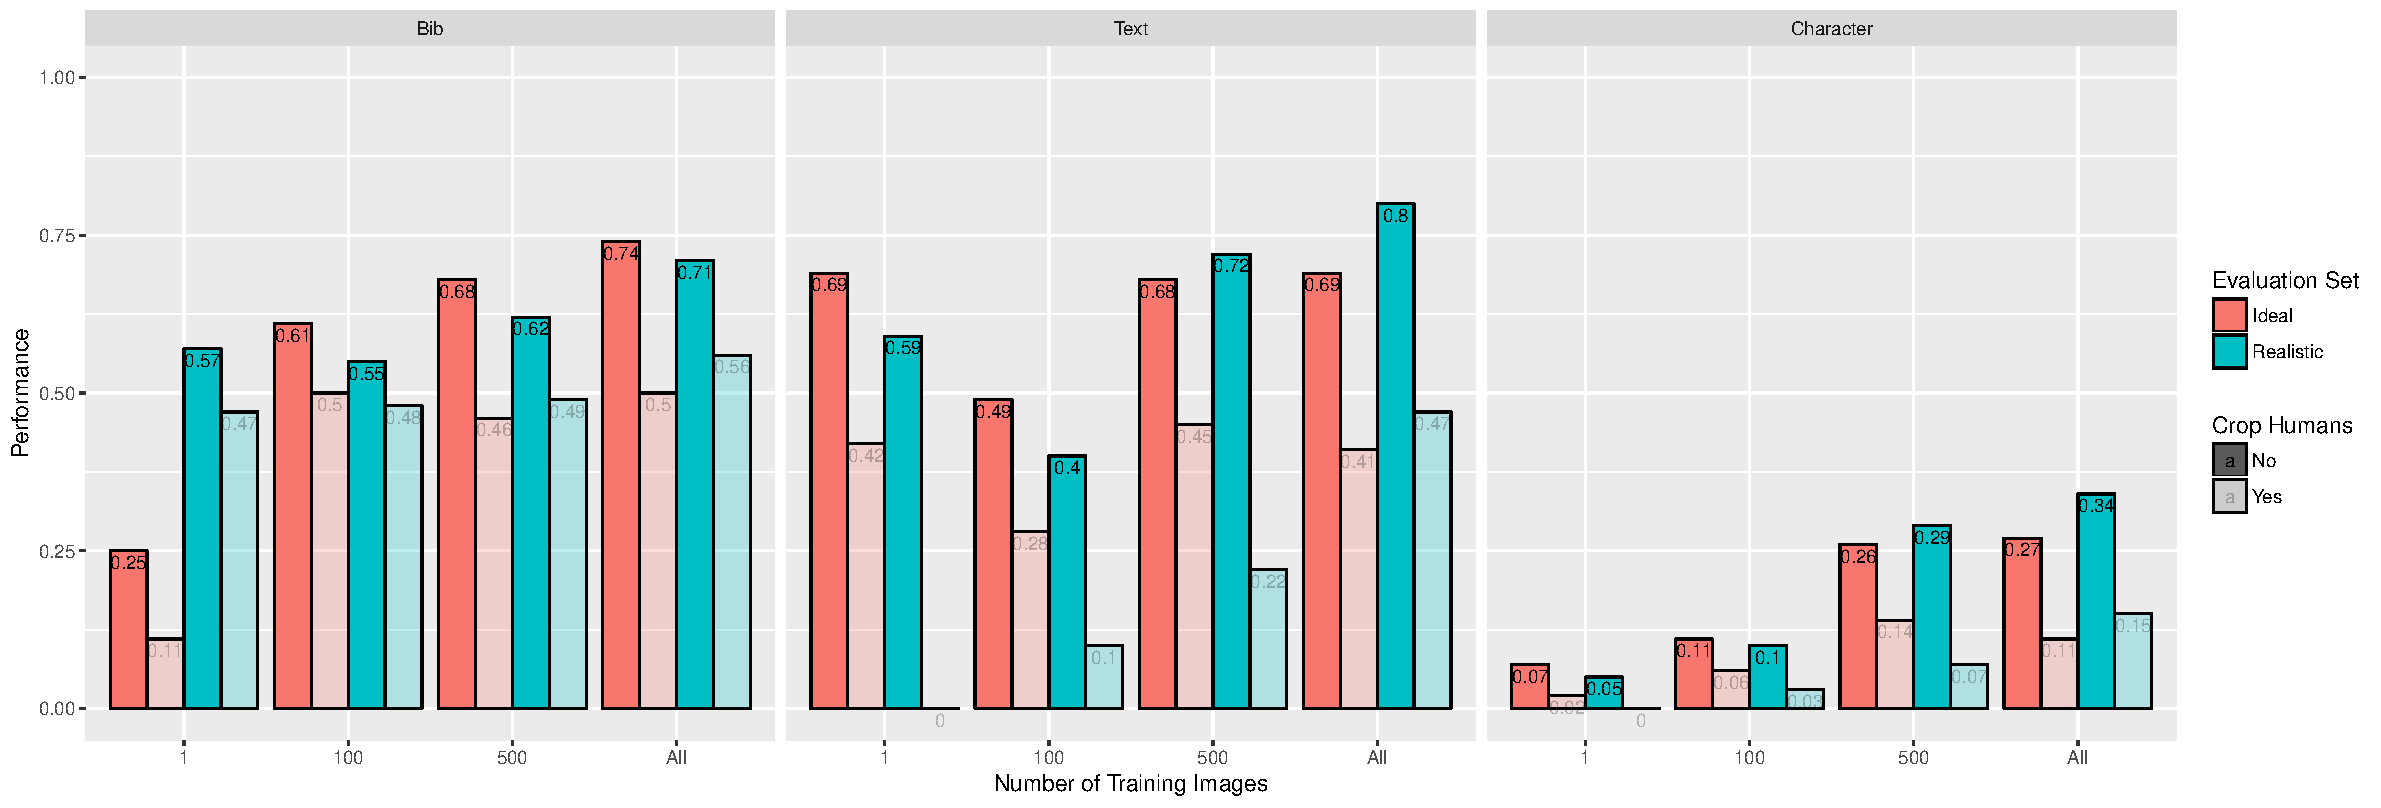
\includegraphics[width=1.15\paperwidth]{images/evaluation/DetectionAll}
  \caption[Bib, text and character performance]{Bib, text and character performance of our pipeline over both realistic and ideal datasets using both cropping and non-cropping.}
  \label{fig:evaluation:results:performance_all}
\end{figure}

\end{landscape}

Thus, the association made by \frcnn{} on the bib sheet to a human torso has a significant impact on the degrading accuracies. A 26\% degrade in performance occurs for bibs which, in turn, has a hinderance on further stages of the pipeline; a 55\% degrade in performance for text occurs and 65\% for character recognition.

The significant decline between text detection and character detection prompted further investigation. We observe in \cref{fig:evaluation:results:performance_all} that the highest bib, text and character performance is generally highest when all training data is used; as the automatic calculation of these stages were not manually verified by a human, we sampled 30 photos twice in two rounds of manual verification for a further evaluation. We discuss this evaluation in the following section.

\subsection{Performance in Manual Evaluation}

A total of 240 photos were manually inspected for both cropping and non-cropping over the ideal and realistic datasets in two rounds\footnote{That is, using all training data, thus evaluation IDs I-ALL-CR, I-ALL-NC, R-ALL-CR, R-ALL-NC.}. Results of both rounds have been averaged in \cref{tab:results:summary:man}, which we present in \cref{fig:evaluation:results:performance_man}.

\begin{figure}[h]
  \centering
  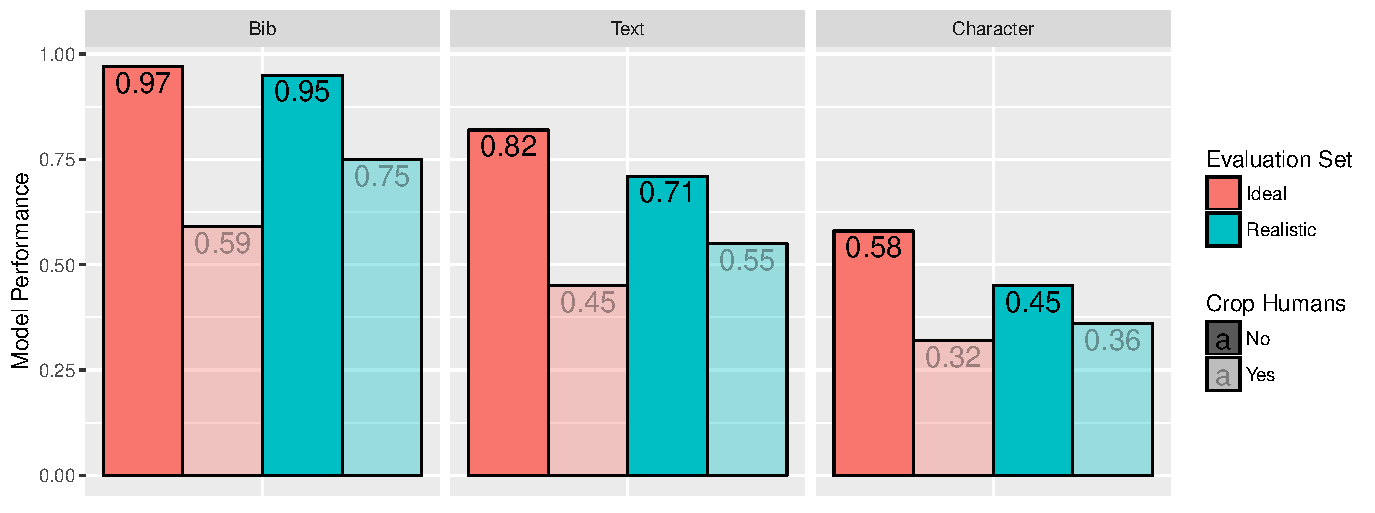
\includegraphics[width=1\textwidth]{images/evaluation/ManualSummary}
  \caption[Bib, text and character performance of manual inspection]{Results of bib, character and text performance manually inspected on a sample of all training images.}
  \label{fig:evaluation:results:performance_man}
\end{figure}

Similar to that of \cref{fig:evaluation:results:performance_all}, a negative association is shown as bib detection progresses to text and character detection. This negative association is clearer in the manual inspection: while bib detection is relatively high for both realistic and ideal cases, there is still a significant drop of performance for cropping and a gradual degrade for stages following bib detection. Character performance still acts as the biggest bottleneck to the pipeline.

In visualising the distribution of our manual evaluation, \citet{wickham:boxplots} show that variations to a boxplot can introduce a richer distributional summary of the histogram or density plot. This retains usefulness in comparing distributions across groups of data. Thus, a violin plot \citep{Hintze:1998fn} is be useful to visualise the density of each individual photo we manually inspected. We present such information in \cref{fig:evaluation:results:mdets_all}\footnote{Jitter has been added to this plot's $y$-axis to improve the plot's readability. The distance between data points in the $y$-axis bears no impact on results and is for aesthetics. Furthermore, the quartiles of each distribution are shown as vertical lines, and the mean of the data points themselves are indicated with the larger solid dot presented alongside with an error bar.} and juxtapose both evaluation sets, comparing cropping versus non-cropping and further conditions of the photo, such as lighting conditions of the photo and the photo's blurriness.

Generally, we observe a wide dichotomy of the individual photo's performance with regards to bib performance. Within realistic non-cropping, we find that all only one photo has a miss-rate of 50\%, with a large cluster toward 100\%. Only two photos have false negatives in the ideal non-cropping case. Text and character detection preserves a similar dichotomy albeit with a larger distribution toward the median in the realistic cases. Most importantly, we see a reflection of our observation that performance in \textit{all models} are improved whereby the mean performances increases from cropping to non-cropping. Generally, there is no bias toward photos taken at night or day as the distribution of both are consistent in all performance categories. Photos that are blurry reflect a poorer performance, and usually fall within the first 25\% of our distribution within all datasets. However, there are some outliers in this case for realistic character performance whereby some blurry photos fall amongst all semi-interquartile ranges. 

To follow up from the character detection performance, we assessed the character recognition performance for true positive cases following this manual evaluation, as described in the following section.

\begin{landscape}

\begin{figure}
  \centering
  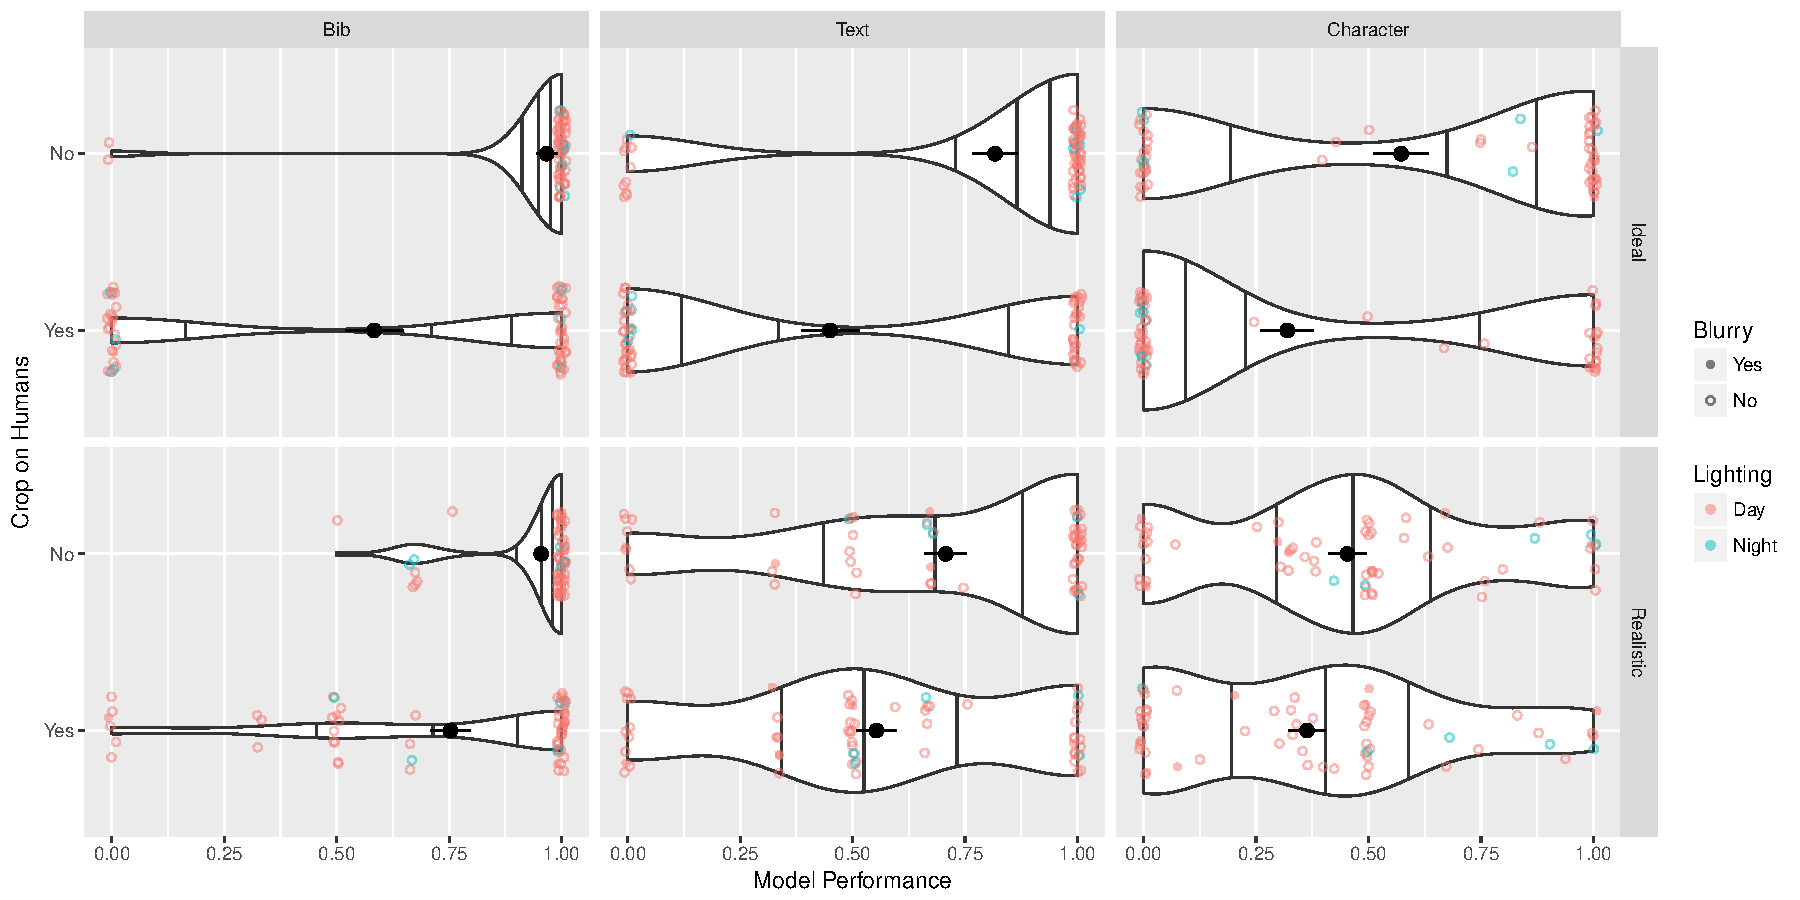
\includegraphics[width=1.20\paperwidth]{images/evaluation/mdets_all}
  \caption[Distribution of manual inspection evaluation]{Distribution of manual evaluation of all 240 photos individually assessed for performance over three categories. We compare the ideal and realistic distribution in the vertical facets whilst also factoring in the photo's lighting and blur conditions.}
  \label{fig:evaluation:results:mdets_all}
\end{figure}

\end{landscape}

\subsection{Overall Performance}

Presented in \cref{fig:evaluation:results:ocr} are the \gls{ocr} performance metrics observed from photos trained with all training data. When compared to \cref{fig:evaluation:metrics:character_rec:sets}, we observe problematic performance in all cases: whilst the pipeline returns true positive matches and some missing false negatives, false positives have been introduced. Cropping shows significicant disadvantages when compared to non-cropping, with a 21\% improvement in true positive matches in realistic cases and 15\% improvement in ideal.

\begin{figure}[h]
  \centering
  \hspace{\fill}
  \begin{subfigure}[b]{0.475\textwidth}
    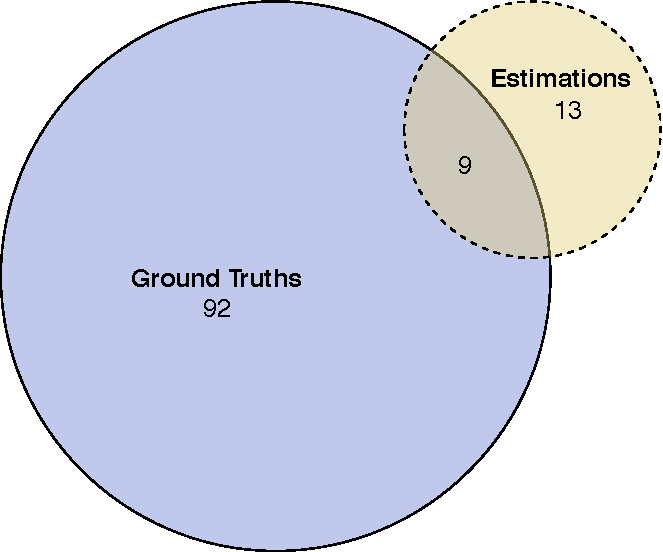
\includegraphics[width=\textwidth]{images/evaluation/ocr_overlap_i_all_cr}
    \caption{I-ALL-CR}
    \label{fig:evaluation:results:ocr:i_all_cr}
  \end{subfigure}
  \hspace{\fill}
  \begin{subfigure}[b]{0.475\textwidth}
    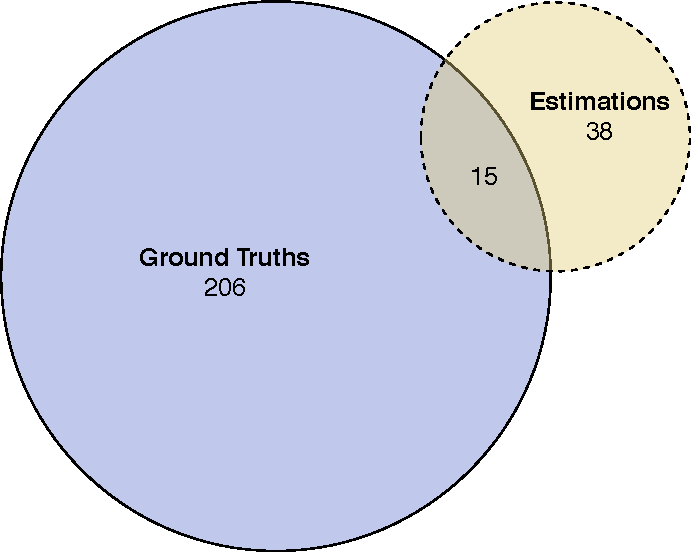
\includegraphics[width=\textwidth]{images/evaluation/ocr_overlap_r_all_cr}
    \caption{R-ALL-CR}
    \label{fig:evaluation:results:ocr:r_all_cr}
  \end{subfigure}
  \hspace{\fill}
  \\
  \bigskip
  \bigskip
  \hspace{\fill}
  \begin{subfigure}[b]{0.475\textwidth}
    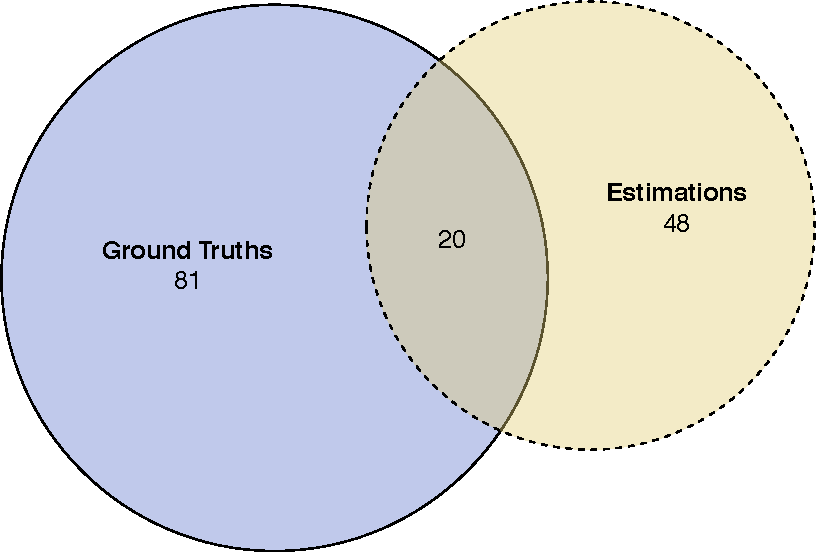
\includegraphics[width=\textwidth]{images/evaluation/ocr_overlap_i_all_nc}
    \caption{I-ALL-NC}
    \label{fig:evaluation:results:ocr:i_all_nc}
  \end{subfigure}
  \hspace{\fill}
  \begin{subfigure}[b]{0.475\textwidth}
    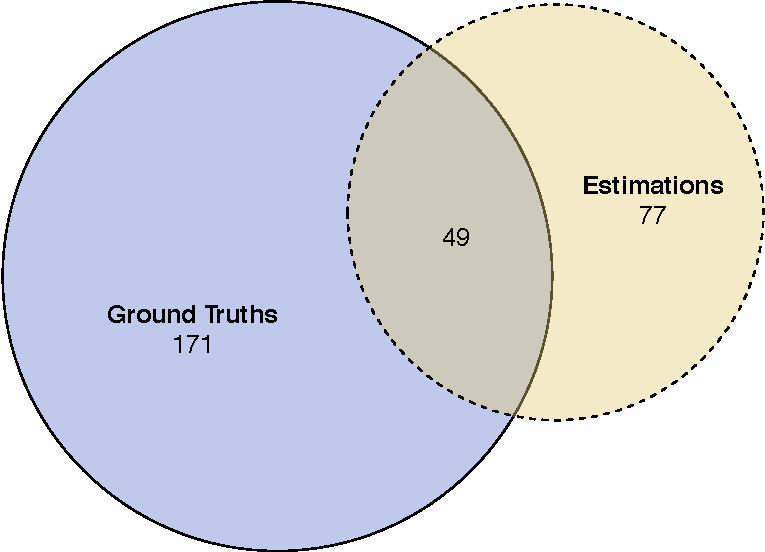
\includegraphics[width=\textwidth]{images/evaluation/ocr_overlap_r_all_nc}
    \caption{R-ALL-NC}
    \label{fig:evaluation:results:ocr:r_all_nc}
  \end{subfigure}
  \hspace{\fill} 
  \bigskip
  \\
  \caption[OCR performance results]{\gls{ocr} performance results of our pipeline on all training data. The first row (subfigures \subref{fig:evaluation:results:ocr:i_all_cr} and \subref{fig:evaluation:results:ocr:r_all_cr}) show ideal/realistic cropping, with a true positive rate of 9 and 7\%, respectively. The second row (subfigures \subref{fig:evaluation:results:ocr:i_all_nc} and \subref{fig:evaluation:results:ocr:r_all_nc}) shows ideal/realistic without cropping, with a true positive rate of 24 and 28\%, respectively.}
  \label{fig:evaluation:results:ocr}
\end{figure}